\chapter{مخططات الجهد--pH}\label{ch:b1:e-ph-diagrams}

يصدأ مسمار من الحديد متروك في ماء المطر؛ والمسمار نفسه في محلول شديد
القاعدية يحتفظ ببريقه أسابيع. ويحمل هيكل السفينة الفولاذي
كتلًا من الزنك تذوب بدلًا منه، وسقف النحاس يخضرّ
لكنه لا يزول أبدًا. مزدوجات أكسدة واختزال يتعلق جهدها بقيمة pH،
وترسيب للهيدروكسيدات والأكاسيد، وتوازنات حمض--قاعدة: الثلاثة كلها
تعمل في آن واحد، وخريطة واحدة تجمعها. فعلى تمثيل للجهد
بدلالة pH، يأخذ كل نوع من أنواع العنصر المنطقة التي يكون فيها هو
الشكل المستقر؛ وقراءة الخريطة تبيّن أي الأنواع يبقى في الماء، وأيها
يتفاعل معًا، وأين يتآكل الفلز.

\begin{recall}
\omterm{thm:b1:nernst:nernst}{معادلة نرنست} \omterm{def:b1:nernst:electrode-potential}{والجهود المعيارية} والتنبؤ بتفاعلات الأكسدة والاختزال
في \cref{ch:b1:nernst}؛ \omterm{def:b1:predominant-reaction:predominance}{ومخططات الغلبة} في
\cref{ch:b1:predominant-reaction}؛ وعتبات ترسيب
الهيدروكسيدات ومناطق وجود الأجسام الصلبة في \cref{ch:b1:precipitation}.
وكل الجهود عند \qty{25}{\celsius}، مع $RT\ln 10/F = \qty{0.059}{V}$.
\end{recall}

\begin{omfigure}
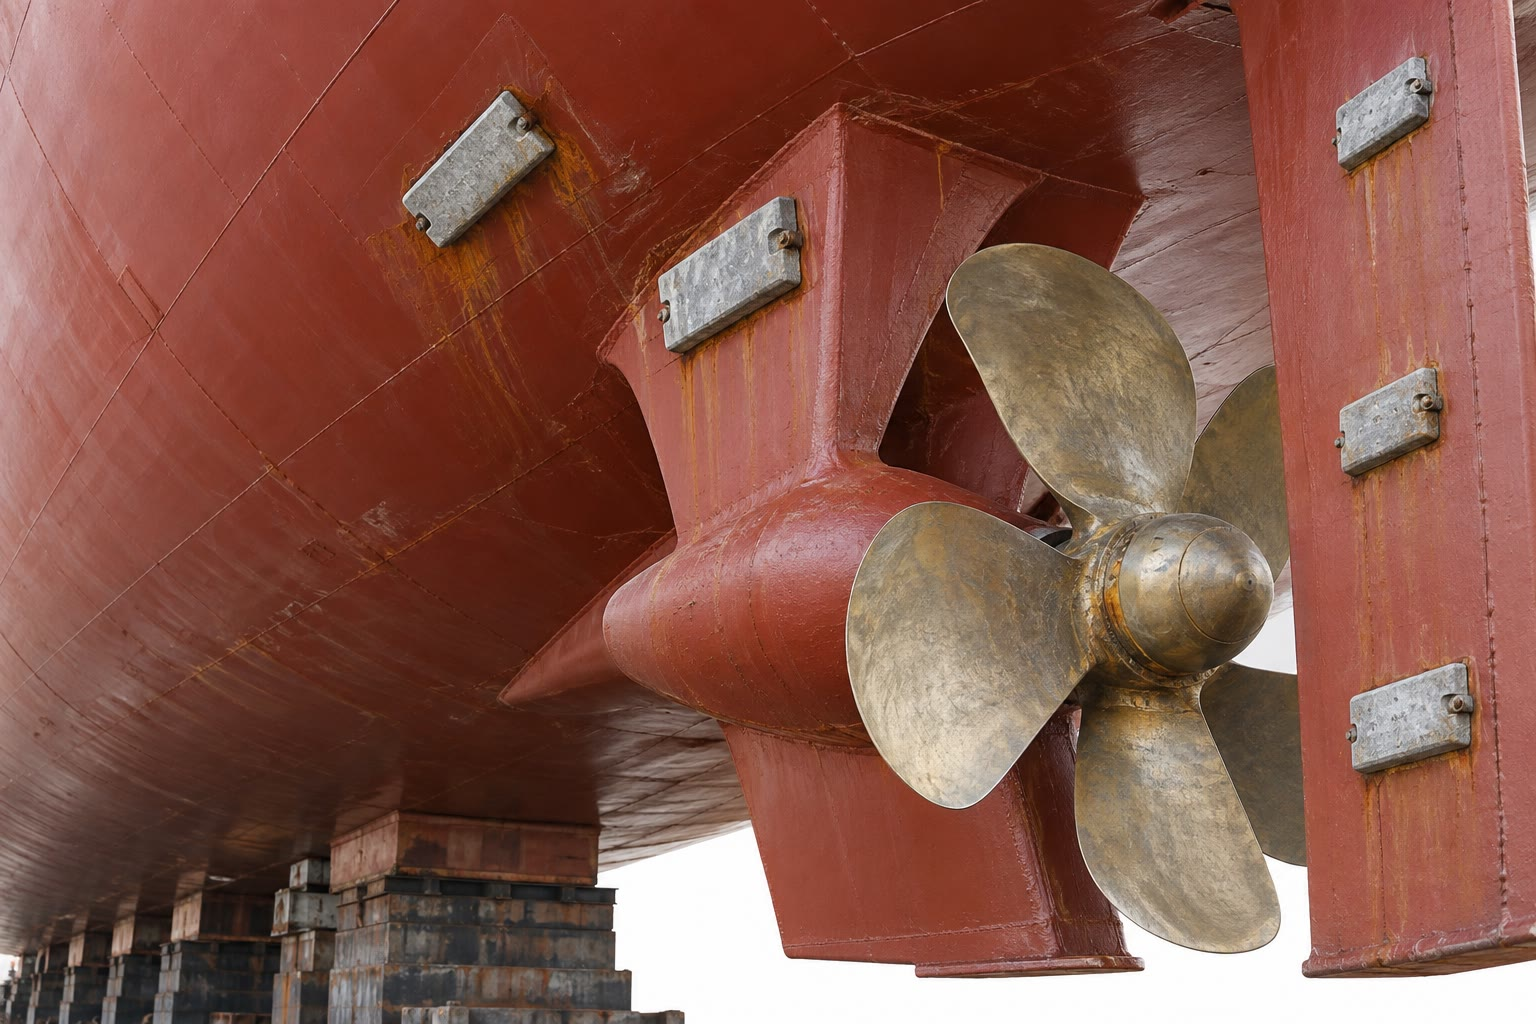
\includegraphics[width=0.6\linewidth]{images/book2/ai/b1-14-ship-anodes.jpg}

{\small مؤخرة سفينة في حوض جاف. الكتل الرمادية المثبتة على الهيكل
قرب المروحة من الزنك: فهي تتآكل في ماء البحر بدلًا من
الفولاذ (\cref{exo:b1:e-ph-diagrams:12}).}
\end{omfigure}

\section{الاصطلاحات}

\begin{definition}[مخطط الجهد--pH، تركيز العمل]\label{def:b1:e-ph-diagrams:e-ph-diagram}
\emph{مخطط الجهد--pH}\index{مخطط الجهد--pH} لعنصر
هو المستوي $(\mathrm{pH}, E)$ مقسَّمًا إلى مناطق، كل منها منطقة
غلبة (للأنواع المذابة) أو \omterm{def:b1:precipitation:existence-domain}{منطقة وجود} (للأجسام الصلبة) لشكل واحد من أشكال
العنصر. ويُرسم من أجل \emph{تركيز
عمل}\index{تركيز العمل} $c$ مختار، هو التركيز الكلي
للعنصر في المحلول، مع هذه الاصطلاحات:
\begin{itemize}
  \item على الحد بين نوعين مذابين، يكون كل منهما بالتركيز $c$
        (معدودًا بذرات العنصر)؛
  \item على الحد بين نوع مذاب وجسم صلب، يكون النوع
        المذاب بالتركيز $c$ والجسم الصلب حاضرًا بالكاد؛
  \item الغازات عند \qty{1}{bar}.
\end{itemize}
وفي هذا الفصل $c = \qty{0.010}{mol/L}$.
\end{definition}

تُرتَّب أشكال العنصر بحسب \omterm{def:b1:nernst:oxidation-number}{عدد الأكسدة}: كلما كبر
العدد علا الشكل في المخطط (فالأشكال المؤكسدة مستقرة عند الجهد
المرتفع). وعند \omterm{def:b1:nernst:oxidation-number}{عدد أكسدة} معطى، تقع الأشكال الأكثر قاعدية
(الهيدروكسيدات، والأكاسيد، \omterm{def:b1:complexation:complex}{والمعقدات} الهيدروكسيلية) إلى اليمين.

\begin{proposition}[ميل الحد]\label{prop:b1:e-ph-diagrams:boundary-slope}
الحد بين نوعين مختلفي \omterm{def:b1:nernst:oxidation-number}{عدد الأكسدة}، تتبادل نصف معادلتهما
$n$ إلكترونًا و$m$ بروتونًا،
$\mathrm{Ox} + m\,\ce{H+} + n\,\mathrm{e^-} \rightleftharpoons \mathrm{Red} +
\cdots$، مستقيم ميله $-0.059\,m/n$ فولت لكل وحدة pH. أما
الحد بين نوعين لهما \omterm{def:b1:nernst:oxidation-number}{عدد الأكسدة} نفسه فرأسي.
\end{proposition}

\begin{proof}
تعطي \omterm{thm:b1:nernst:nernst}{معادلة نرنست} $E = E^\circ + \frac{0.059}{n}\log\frac{[\mathrm{Ox}]
[\ce{H+}]^m}{[\mathrm{Red}]} = E^\circ + \frac{0.059}{n}\log\frac{[\mathrm{Ox}]}
{[\mathrm{Red}]} - \frac{0.059\,m}{n}\,\mathrm{pH}$، وعلى الحد تكون
التراكيز محددة بالاصطلاحات. ويرتبط نوعان لهما \omterm{def:b1:nernst:oxidation-number}{عدد
الأكسدة} نفسه بتوازن حمض--قاعدة أو ترسيب
دون إلكترونات، يحدد ثابته قيمة pH للحد
مهما كان الجهد.
\end{proof}

\section{الماء}

\begin{proposition}[مستقيما الماء]\label{prop:b1:e-ph-diagrams:water-lines}
تحت \qty{1}{bar} من الغاز، يُختزل الماء إلى هيدروجين تحت المستقيم
$E = -0.059\,\mathrm{pH}$ ويتأكسد إلى أكسجين فوق المستقيم $E = 1.23
- 0.059\,\mathrm{pH}$.
\end{proposition}

\begin{proof}
\ce{2H+ + 2e- -> H2}: $E = 0 + \frac{0.059}{2}\log\frac{[\ce{H+}]^2}{p(\ce{H2})}
= -0.059\,\mathrm{pH}$ عند $p = 1$. \ce{O2 + 4H+ + 4e- -> 2H2O}: $E = 1.23 +
\frac{0.059}{4}\log(p(\ce{O2})[\ce{H+}]^4) = 1.23 - 0.059\,\mathrm{pH}$. وتحت
المستقيم الأول يكون \ce{H2} هو الشكل المستقر للمزدوجة (فيُختزل
الماء)؛ وفوق الثاني يكون \ce{O2} هو المستقر.
\end{proof}

\begin{definition}[منطقة استقرار الماء]\label{def:b1:e-ph-diagrams:water-domain}
الشريط بين المستقيمين، الذي عرضه \qty{1.23}{V} عند كل pH، هو
\emph{منطقة استقرار الماء}\index{منطقة استقرار الماء}: فالنوع
الذي تقع منطقته كلها داخله لا يؤكسد الماء ولا
يختزله.
\end{definition}

\section{بناء مخطط: الحديد}

\begin{method}[بناء مخطط الجهد--pH]\label{met:b1:e-ph-diagrams:build}
\begin{enumerate}
  \item عدّد الأنواع ورتّبها بحسب \omterm{def:b1:nernst:oxidation-number}{عدد الأكسدة}: في الحديد،
        \ce{Fe} (0)، و\ce{Fe^2+} و\ce{Fe(OH)2} (\babelsublr{$+$II})، و\ce{Fe^3+}
        و\ce{Fe(OH)3} (\babelsublr{$+$III}).
  \item عند كل \omterm{def:b1:nernst:oxidation-number}{عدد أكسدة}، أوجد الحدود الرأسية من
        توازنات الترسيب (أو الحمض--القاعدة) عند \omterm{def:b1:e-ph-diagrams:e-ph-diagram}{تركيز
        العمل} (\cref{ch:b1:precipitation}).
  \item لكل زوج من \omterm{def:b1:nernst:oxidation-number}{أعداد الأكسدة} المتجاورة، اكتب
        \omterm{def:b1:nernst:couple}{نصف المعادلة} في كل مجال من مجالات pH \omterm{thm:b1:nernst:nernst}{ومعادلة نرنست} الخاصة بها مع
        الاصطلاحات؛ فيعطي ذلك حدًا مستقيمًا معلوم الميل.
  \item اجمع المستقيمات من اليسار إلى اليمين؛ وحيث تلتقي ثلاثة مستقيمات،
        لا يستمر كل منها إلا في الجهة التي يكون فيها نوعاه كلاهما
        مستقرين.
  \item تحقق: يجب ألا تتداخل المناطق، ويجب أن تتفق الميول
        مع \cref{prop:b1:e-ph-diagrams:boundary-slope}.
\end{enumerate}
\end{method}

\begin{example}[حدود الحديد]\label{ex:b1:e-ph-diagrams:iron}
مع $c = \qty{0.010}{mol/L}$ (وثوابت \cref{ch:b1:precipitation,ch:b1:nernst}):
\begin{itemize}
  \item $\ce{Fe^3+}/\ce{Fe(OH)3}$: $\mathrm{pH} = 14.00 - \frac13(38.55 - 2) = 1.82$؛
        $\ce{Fe^2+}/\ce{Fe(OH)2}$: $\mathrm{pH} = 14.00 - \frac12(16.31 - 2) = 6.85$.
  \item $\ce{Fe^2+}/\ce{Fe}$: $E = -0.41 + 0.030\log c = -0.47$~V (من أجل pH أدنى من 6.85).
  \item $\ce{Fe^3+}/\ce{Fe^2+}$: $E = 0.77$~V (كلاهما بالتركيز $c$، من أجل pH أدنى من 1.82).
  \item $\ce{Fe(OH)3}/\ce{Fe^2+}$: \ce{Fe(OH)3 + 3H+ + e- -> Fe^2+ + 3H2O}، والميل
        $-0.177$: $E = 1.09 - 0.177\,\mathrm{pH}$ بين pH 1.82 و6.85.
  \item $\ce{Fe(OH)3}/\ce{Fe(OH)2}$: إلكترون واحد، وبروتون واحد، $E = 0.28 -
        0.059\,\mathrm{pH}$؛ $\ce{Fe(OH)2}/\ce{Fe}$: إلكترونان، وبروتونان،
        $E = -0.07 - 0.059\,\mathrm{pH}$ (من أجل pH أعلى من 6.85).
\end{itemize}
وتُستخرج القيم عند المبدأ بالاتصال عند النقاط الثلاثية، أو
مباشرة من طاقات غيبس للتكوين؛ والمخطط أدناه
محسوب من هذه الأخيرة، وتختلف حدوده عن هذه القيم المقرَّبة
بأقل من \qty{0.01}{V} أو 0.01 وحدة pH.
% ledger: dfg:Fe2+_ao, dfg:Fe3+_ao, dfg:Fe_OH2_cr, dfg:Fe_OH3_cr, dfg:H2O_l, dfg:OH-_ao (boundaries computed in figdata/bachelor-1/eph-diagrams.py)
\end{example}

\begin{omfigure}
\begin{tikzpicture}
\begin{axis}[
  width=0.8\linewidth, height=8.2cm, xmin=0, xmax=14, ymin=-1.2, ymax=1.6,
  axis x line=bottom, axis y line=left, xlabel={\babelsublr{pH}}, ylabel={\babelsublr{$E$ (V)}},
  xtick={0,2,4,6,8,10,12,14}, ytick={-1,-0.5,0,0.5,1,1.5},
  unbounded coords=jump, clip=true,
  tick label style={font=\small}, label style={font=\small}]
\addplot[black!45, dashed] table[x=pH, y=H2] {figdata/out/bachelor-1-eph-diagrams-water.dat};
\addplot[black!45, dashed] table[x=pH, y=O2] {figdata/out/bachelor-1-eph-diagrams-water.dat};
\addplot[omDef, very thick] table[x=pH, y=E] {figdata/out/bachelor-1-eph-diagrams-iron.dat};
\node[font=\small] at (axis cs:3.2,-0.85) {\ce{Fe}};
\node[font=\small] at (axis cs:3.4,0.15) {\ce{Fe^2+}};
\node[font=\small] at (axis cs:0.9,1.45) {\ce{Fe^3+}};
\node[font=\small] at (axis cs:8.5,0.25) {\ce{Fe(OH)3}};
\node[font=\scriptsize] at (axis cs:11.0,-0.56) {\ce{Fe(OH)2}};
\node[font=\scriptsize, black!55, rotate=-14, anchor=south] at (axis cs:12.0,0.52) {\ce{O2}/\ce{H2O}};
\node[font=\scriptsize, black!55, rotate=-14, anchor=south] at (axis cs:2.2,-0.11) {\ce{H2O}/\ce{H2}};
\end{axis}
\end{tikzpicture}

{\small \omterm{def:b1:e-ph-diagrams:e-ph-diagram}{مخطط الجهد--pH} للحديد من أجل $c = \qty{0.010}{mol/L}$ (الخطوط
المتصلة)، مع مستقيمي الماء (المتقطعين). وكل حد محسوب
من طاقات غيبس المجدولة للتكوين.}
\end{omfigure}

\section{النحاس والزنك}

تعطي الطريقة نفسها مخططي النحاس (الأنواع \ce{Cu}، و\ce{Cu+}،
و\ce{Cu2O} عند \babelsublr{$+$I}، و\ce{Cu^2+}، و\ce{CuO} عند \babelsublr{$+$II}) والزنك (\ce{Zn}،
و\ce{Zn^2+}، و\ce{Zn(OH)2}، و\ce{Zn(OH)4^2-}). ففي النحاس يظهر \ce{CuO}
عند $\mathrm{pH} = 14.00 - \frac12(20.64 - 2) = 4.68$، وأيون \ce{Cu+}، وإن ورد في القائمة، ليست له
أي منطقة: ففي الحمض يقع $E^\circ(\ce{Cu+}/\ce{Cu}) = 0.52$~V فوق
$E^\circ(\ce{Cu^2+}/\ce{Cu+}) = 0.16$~V، فتُشطب منطقته المفترضة
بجاريه (\cref{sec:b1:e-ph-diagrams:reading}).
وفي الزنك يظهر الهيدروكسيد عند pH 6.81 ولا يعود إلى الذوبان على هيئة
\ce{Zn(OH)4^2-} إلا فوق 13.97 عند هذا التركيز، أي شريحة رقيقة عند
الحافة اليمنى.

\begin{omfigure}
\begin{tikzpicture}
\begin{axis}[name=cu,
  width=0.47\linewidth, height=7cm, xmin=0, xmax=14, ymin=-1.4, ymax=1.6,
  axis x line=bottom, axis y line=left, xlabel={\babelsublr{pH}}, ylabel={\babelsublr{$E$ (V)}},
  xtick={0,4,8,12}, ytick={-1,-0.5,0,0.5,1,1.5},
  unbounded coords=jump, clip=true,
  tick label style={font=\small}, label style={font=\small}]
\addplot[black!45, dashed] table[x=pH, y=H2] {figdata/out/bachelor-1-eph-diagrams-water.dat};
\addplot[black!45, dashed] table[x=pH, y=O2] {figdata/out/bachelor-1-eph-diagrams-water.dat};
\addplot[omDef, very thick] table[x=pH, y=E] {figdata/out/bachelor-1-eph-diagrams-copper.dat};
\node[font=\small] at (axis cs:5,-0.7) {\ce{Cu}};
\node[font=\small] at (axis cs:2,0.7) {\ce{Cu^2+}};
\node[font=\small] at (axis cs:9.5,0.75) {\ce{CuO}};
\node[font=\scriptsize] (cuo) at (axis cs:11.8,-1.05) {\ce{Cu2O}};
\draw[->, black!70] (cuo.north) -- (axis cs:10,-0.035);
\node[font=\small, anchor=north] at (axis cs:7,1.58) {النحاس};
\end{axis}
\begin{axis}[at={(cu.east)}, anchor=west, xshift=1.5cm,
  width=0.47\linewidth, height=7cm, xmin=0, xmax=14, ymin=-1.4, ymax=1.6,
  axis x line=bottom, axis y line=left, xlabel={\babelsublr{pH}}, ylabel={\babelsublr{$E$ (V)}},
  xtick={0,4,8,12}, ytick={-1,-0.5,0,0.5,1,1.5},
  unbounded coords=jump, clip=true,
  tick label style={font=\small}, label style={font=\small}]
\addplot[black!45, dashed] table[x=pH, y=H2] {figdata/out/bachelor-1-eph-diagrams-water.dat};
\addplot[black!45, dashed] table[x=pH, y=O2] {figdata/out/bachelor-1-eph-diagrams-water.dat};
\addplot[omDef, very thick] table[x=pH, y=E] {figdata/out/bachelor-1-eph-diagrams-zinc.dat};
\node[font=\small] at (axis cs:3.5,-1.15) {\ce{Zn}};
\node[font=\small] at (axis cs:3.2,0.4) {\ce{Zn^2+}};
\node[font=\small] at (axis cs:10.2,0.4) {\ce{Zn(OH)2}};
\draw[->] (axis cs:12.4,1.15) node[left, font=\scriptsize] {\ce{Zn(OH)4^2-}} -- (axis cs:13.95,1.15);
\node[font=\small, anchor=north] at (axis cs:10.5,1.58) {الزنك};
\end{axis}
\end{tikzpicture}

{\small مخططا الجهد--pH للنحاس والزنك ($c =
\qty{0.010}{mol/L}$)، مع مستقيمي الماء (المتقطعين). منطقة
فلز النحاس تتداخل مع منطقة الماء؛ أما منطقة الزنك فتقع كلها
تحت مستقيم الهيدروجين.}
% ledger: dfg:Cu+_ao, dfg:Cu2+_ao, dfg:Cu2O_cr, dfg:CuO_cr, dfg:Zn2+_ao, dfg:Zn_OH2_cr, dfg:Zn_OH42-_ao (boundaries computed in figdata/bachelor-1/eph-diagrams.py)
\end{omfigure}

\section{قراءة مخطط}\label{sec:b1:e-ph-diagrams:reading}

\begin{proposition}[المناطق المنفصلة]\label{prop:b1:e-ph-diagrams:disjoint-domains}
إذا كانت منطقة \omterm{def:b1:nernst:couple}{مؤكسد}، عند pH معطى، تقع كلها فوق منطقة
\omterm{def:b1:nernst:couple}{مختزل}، دون جزء مشترك، تفاعل الاثنان؛ أما الأنواع التي
تشترك مناطقها في منطقة ما فيمكن أن تتعايش في \omterm{def:b1:extent-q-and-k:quantitative}{حالة توازن}.
\end{proposition}

\begin{proof}
عند ذلك pH، يكون لمزدوجة \omterm{def:b1:nernst:couple}{المؤكسد} فوق حدها جهد
أعلى من أي جهد تبلغه مزدوجة \omterm{def:b1:nernst:couple}{المختزل}: فوفق
\cref{prop:b1:nernst:equilibrium-constant} يكون للتفاعل بينهما
$K > 1$، ويستمر حتى يُستهلك أحدهما أو تلتقي
منطقتاهما. أما داخل منطقة مشتركة فكلاهما الشكلان المستقران عند
الجهد نفسه: فلا شيء يدفع إلى تفاعل.
\end{proof}

الحديد والماء: منطقة فلز الحديد تقع تحت المستقيم
$\ce{H2O}/\ce{H2}$ عند كل pH. فالحديد يختزل الماء، في المحلول الحمضي
مع انطلاق مرئي للهيدروجين؛ ومع الأكسجين المذاب يتأكسد
أسرع أيضًا. النحاس: منطقته تتداخل مع منطقة الماء، فلا يختزل النحاس
الماء ولا الأحماض التي ليست هي نفسها مؤكسدة، لكن
أكسجين الهواء، الواقع فوقه، يؤكسده ببطء --- والزنجار الأخضر على الأسقف
ناتج لاحق لتلك الأكسدة مع ثنائي أكسيد الكربون ومركبات
الكبريت. فالمخطط يقول ما هو ممكن، لا مدى سرعته: فكثير من التفاعلات
التي يسمح بها بطيئة، وهي مسألة يعالجها مجلد السنة الثانية.

\begin{definition}[عدم التناسب، التناسب]\label{def:b1:e-ph-diagrams:disproportionation}
\emph{عدم التناسب}\index{عدم التناسب} هو تفاعل
نوع مع نفسه، يتأكسد جزء منه ويُختزل الجزء الآخر:
\ce{2Cu+ -> Cu^2+ + Cu}. وعكسه، أي إعطاء نوعين من العنصر نفسه
نوعًا ذا \omterm{def:b1:nernst:oxidation-number}{عدد أكسدة} وسيط، هو
\emph{التناسب}\index{تناسب}:
\ce{2Fe^3+ + Fe -> 3Fe^2+}.
\end{definition}

\begin{proposition}[معيار عدم التناسب]\label{prop:b1:e-ph-diagrams:disproportionation-criterion}
يخضع النوع B ذو \omterm{def:b1:nernst:oxidation-number}{عدد الأكسدة} الوسيط، في المزدوجتين A/B
وB/C، \omterm{def:b1:e-ph-diagrams:disproportionation}{لعدم التناسب} إذا كان $E(\mathrm{B}/\mathrm{C}) > E(\mathrm{A}/\mathrm{B})$:
فلا تكون له عندئذ منطقة خاصة به، ويحل حد واحد A/C محل
الحدين.
\end{proposition}

\begin{proof}
B هو \omterm{def:b1:nernst:couple}{مؤكسد} المزدوجة B/C \omterm{def:b1:nernst:couple}{ومختزل} المزدوجة A/B. فإذا وقعت المزدوجة B/C
فوق A/B، جعلت قاعدة غاما (\cref{met:b1:nernst:predict-redox}) النوع B
(\omterm{def:b1:nernst:couple}{المؤكسد}، المزدوجة العليا) يتفاعل مع B (\omterm{def:b1:nernst:couple}{المختزل}، المزدوجة السفلى)، معطيًا C
وA. وهندسيًا، لا يكون B مستقرًا إلا فوق $E(\mathrm{B}/\mathrm{C})$
وتحت $E(\mathrm{A}/\mathrm{B})$، وهذه مجموعة خالية.
\end{proof}

\begin{definition}[مناطق المناعة والتآكل والتخميل]\label{def:b1:e-ph-diagrams:corrosion-domains}
على مخطط فلز، تكون منطقة الفلز نفسه
\emph{منطقة مناعته}\index{منطقة المناعة} (فلا يمكن أن يتأكسد)؛
وتكوّن مناطق أيوناته المذابة \emph{منطقة
التآكل}\index{منطقة التآكل}؛ وتكوّن مناطق أكاسيده
وهيدروكسيداته الصلبة، التي قد تكسو الفلز، \emph{منطقة
التخميل}\index{منطقة التخميل}. أما هل تحمي الكسوة حقًا
الفلز فمسألة حركية، يعالجها مجلد السنة الثانية.
\end{definition}

\begin{method}[قراءة مخطط]\label{met:b1:e-ph-diagrams:read}
\begin{enumerate}
  \item ضع مستقيمي الماء فوق المخطط: النوع الذي تقع منطقته خارج
        شريط الماء يتفاعل مع الماء (ترموديناميكيًا).
  \item لنوعين من عنصرين مختلفين، ضع مخططيهما أحدهما فوق الآخر:
        فالمناطق المنفصلة عند pH المعني تعني تفاعلًا.
  \item في الفلز، حدّد موضع النقطة (pH، $E$) للوسط: مناعة، أو
        تآكل، أو تخميل.
  \item تذكّر أن المخطط مرسوم \omterm{def:b1:e-ph-diagrams:e-ph-diagram}{لتركيز عمل} واحد؛
        وأن الحدود مع الأنواع المذابة تنزاح بمقدار $0.059/n$~V لكل
        عشرة أضعاف في التركيز.
\end{enumerate}
\end{method}

الزنك يحمي الحديد: في ماء البحر (pH نحو 8) يتماس زنك الهيكل
وفولاذه؛ فيتأكسد الزنك، ذو الجهد الأدنى، أولًا وتُبقي
الإلكترونات التي يحررها الحديدَ في \omterm{def:b1:e-ph-diagrams:corrosion-domains}{منطقة مناعته} أو قربها.
وتُستهلك كتلة الزنك وتُستبدل في كل دخول إلى الحوض الجاف.

\section{تمارين}

\begin{exercise}[$\star$]\label{exo:b1:e-ph-diagrams:1}
رتّب بحسب \omterm{def:b1:nernst:oxidation-number}{عدد أكسدة} العنصر الأنواع \ce{Mn} و\ce{Mn^2+}
و\ce{MnO2} و\ce{MnO4-} و\ce{Mn(OH)2}، و\ce{Cl-} و\ce{Cl2} و\ce{HClO}
و\ce{ClO-} و\ce{ClO3-}.
\end{exercise}

\begin{exercise}[$\star$]\label{exo:b1:e-ph-diagrams:2}
أعطِ ميل الحد لكل \omterm{def:b1:nernst:couple}{نصف معادلة}:
\ce{Fe(OH)3 + 3H+ + e- -> Fe^2+ + 3H2O}؛ \ce{2Cu^2+ + H2O + 2e- -> Cu2O + 2H+}؛
\ce{MnO4- + 8H+ + 5e- -> Mn^2+ + 4H2O}؛ \ce{Zn(OH)2 + 2H+ + 2e- -> Zn + 2H2O}.
لماذا كان ميل إحداها موجبًا؟
\end{exercise}

\begin{exercise}[$\star$]\label{exo:b1:e-ph-diagrams:3}
عند أي pH يمر مستقيما الماء بالقيمة 0~V وبالقيمة
\qty{0.50}{V}؟ وما عرض \omterm{def:b1:e-ph-diagrams:water-domain}{منطقة استقرار الماء} عند
pH 7؟
\end{exercise}

\begin{exercise}[$\star$]\label{exo:b1:e-ph-diagrams:4}
مستعينًا بمخطط الحديد، أعطِ الشكل المستقر للحديد عند
(pH 1، $E = 1.0$~V)، و(pH 4، $E = 0$)، و(pH 10، $E = -0.4$~V)
و(pH 10، $E = 0.5$~V).
\end{exercise}

\begin{exercise}[$\star\star$]\label{exo:b1:e-ph-diagrams:5}
أعد حساب الحد $\ce{Fe^2+}/\ce{Fe}$ والحد الرأسي
$\ce{Fe^3+}/\ce{Fe(OH)3}$ من أجل \omterm{def:b1:e-ph-diagrams:e-ph-diagram}{تركيز عمل} قدره
\qty{1.0e-6}{mol/L}، وهي القيمة المستعملة في مناقشة التآكل. أي المناطق
يتسع؟
\end{exercise}

\begin{exercise}[$\star\star$]\label{exo:b1:e-ph-diagrams:6}
استنتج الحد $\ce{Fe(OH)3}/\ce{Fe^2+}$: اكتب \omterm{def:b1:nernst:couple}{نصف المعادلة}،
\omterm{thm:b1:nernst:nernst}{ومعادلة نرنست} الخاصة بها، واستعمل الاتصال عند pH 1.82 لتبيّن أن $E = 1.09 -
0.177\,\mathrm{pH}$.
\end{exercise}

\begin{exercise}[$\star\star$]\label{exo:b1:e-ph-diagrams:7}
بيّن مستعينًا بجدول \omterm{def:b1:nernst:electrode-potential}{الجهود المعيارية} أن \ce{Cu+} يخضع \omterm{def:b1:e-ph-diagrams:disproportionation}{لعدم التناسب}
عند pH 0 وأعطِ جهد الحد الوحيد $\ce{Cu^2+}/\ce{Cu}$
عند $c = \qty{0.010}{mol/L}$.
\end{exercise}

\begin{exercise}[$\star\star$]\label{exo:b1:e-ph-diagrams:8}
هل يذوب النحاس في حمض الكلوريدريك عند pH 0 بمعزل عن الهواء؟ وفي حمض
النتريك (المزدوجة $\ce{NO3-}/\ce{NO}$، $E^\circ = 0.96$~V)؟ علّل بالمخطط
والجهود.
\end{exercise}

\begin{exercise}[$\star\star$]\label{exo:b1:e-ph-diagrams:9}
تصير محاليل الحديد(II) المتروكة في الهواء صفراء بنية. فسّر بمخطط
الحديد والمستقيم $\ce{O2}/\ce{H2O}$، واكتب التفاعل عند pH 3.
\end{exercise}

\begin{exercise}[$\star\star\star$]\label{exo:b1:e-ph-diagrams:10}
ابنِ مخطط الزنك من أجل $c = \qty{0.010}{mol/L}$: احسب
الحدين الرأسيين عند pH 6.81 و13.97، والحد $\ce{Zn^2+}/\ce{Zn}$،
ومعادلتي $\ce{Zn(OH)2}/\ce{Zn}$ و$\ce{Zn(OH)4^2-}/\ce{Zn}$.
\end{exercise}

\begin{exercise}[$\star\star\star$]\label{exo:b1:e-ph-diagrams:11}
ضع مخطط الحديد فوق مخطط الماء وناقش مصير مسمار
حديد في ماء منزوع الأكسجين عند pH 2، وعند pH 7 وعند pH 13. ماذا
يتغير مع الأكسجين المذاب؟
\end{exercise}

\begin{exercise}[$\star\star\star$]\label{exo:b1:e-ph-diagrams:12}
المصاعد التضحوية. يوصل هيكل فولاذي في ماء البحر (pH 8) بكتلة
من الزنك. مستعينًا بالمخططات، فسّر أي الفلزين يتأكسد، واكتب
التفاعلات مع الأكسجين المذاب، وبيّن لماذا ينفع المغنيسيوم أيضًا
ولماذا يزيد النحاس الأمر سوءًا.
\end{exercise}

\section{مسألة: ماء جافيل والمسبح}

\begin{problem}[{مسألة نهاية الأسبوع --- \omterm{def:b1:nernst:oxidation-number}{أعداد أكسدة} الكلور،
والمزدوجة حمض--قاعدة HClO/ClO\textsuperscript{$-$}، \omterm{def:b1:e-ph-diagrams:e-ph-diagram}{ومخطط الجهد--pH}
للكلور، وقيمة pH التي يخضع فوقها الكلور المذاب \omterm{def:b1:e-ph-diagrams:disproportionation}{لعدم التناسب}}]
\label{pb:b1:e-ph-diagrams:1}
ماء جافيل محلول قاعدي من هيبوكلوريت الصوديوم وكلوريد الصوديوم؛
ويُطهَّر المسبح بحمض الهيبوكلوروز الذي يحويه، عند
pH مُبقًى أعلى قليلًا من 7. وخلط ماء جافيل بمنظف حمضي يحرر
غاز الكلور. معطيات عند \qty{25}{\celsius}: $E^\circ(\ce{Cl2(aq)}/\ce{Cl-})
= 1.396$~V، $E^\circ(\ce{HClO}/\ce{Cl2(aq)}) = 1.594$~V،
$\mathrm{p}K_a(\ce{HClO}/\ce{ClO-}) = 7.55$، $RT\ln 10/F = 0.0592$~V؛
\omterm{def:b1:e-ph-diagrams:e-ph-diagram}{وتركيز العمل} $c = \qty{0.010}{mol/L}$ من ذرات الكلور.

\medskip
\noindent\textbf{الجزء الأول --- الأنواع.}
\begin{enumerate}
  \item أعطِ \omterm{def:b1:nernst:oxidation-number}{عدد أكسدة} الكلور في \ce{Cl-} و\ce{Cl2}
        و\ce{HClO} و\ce{ClO-}.
  \item رتّب الأنواع الأربعة على محور رأسي \omterm{def:b1:nernst:oxidation-number}{لعدد الأكسدة}.
  \item أي النوعين لهما \omterm{def:b1:nernst:oxidation-number}{عدد الأكسدة} نفسه؟ وما العلاقة
        بينهما؟
  \item اكتب \omterm{def:b1:nernst:couple}{نصف معادلة} $\ce{Cl2}/\ce{Cl-}$.
  \item اكتب \omterm{def:b1:nernst:couple}{نصف معادلة} $\ce{HClO}/\ce{Cl2}$.
  \item اكتب \omterm{def:b1:nernst:couple}{نصف معادلة} $\ce{ClO-}/\ce{Cl-}$ في محلول قاعدي.
\end{enumerate}

\medskip
\noindent\textbf{الجزء الثاني --- حمض الهيبوكلوروز.}
\begin{enumerate}[resume]
  \item ارسم \omterm{def:b1:predominant-reaction:predominance}{مخطط الغلبة} للنوعين \ce{HClO} و\ce{ClO-} بدلالة
        pH.
  \item لماذا كان حدهما على \omterm{def:b1:e-ph-diagrams:e-ph-diagram}{مخطط الجهد--pH} رأسيًا؟
  \item احسب كسر حمض الهيبوكلوروز عند pH 7.4.
  \item الأمر نفسه عند pH 8.0. حمض الهيبوكلوروز هو المطهِّر الأفضل: فلماذا
        يمنع مشغّلو المسابح pH من الانجراف صعودًا إلى 8؟
  \item في ماء جافيل (pH نحو 12)، أي الشكلين حاضر؟
\end{enumerate}

\medskip
\noindent\textbf{الجزء الثالث --- المخطط.}
باصطلاحات الفصل، يكون \ce{Cl2(aq)} بالتركيز $c/2$
و\ce{Cl-} و\ce{HClO} و\ce{ClO-} بالتركيز $c$ على الحد.
\begin{enumerate}[resume]
  \item بيّن أن الحد $\ce{Cl2}/\ce{Cl-}$ يقع عند $E = 1.396 +
        0.0296\log\bigl((c/2)/c^2\bigr) = 1.446$~V، مستقلًا عن pH.
  \item بيّن أن الحد $\ce{HClO}/\ce{Cl2}$ هو $E = 1.594 -
        0.0296\log 50 - 0.0592\,\mathrm{pH} \approx 1.544 -
        0.0592\,\mathrm{pH}$.
  \item أوجد قيمة pH التي يتقاطع عندها هذان المستقيمان.
  \item بعد هذه القيمة يكون الحد $\ce{HClO}/\ce{Cl-}$. اكتب
        نصف معادلته وبيّن أن ميله $-0.0296$.
  \item احسب $E^\circ(\ce{HClO}/\ce{Cl-})$ من الجهدين المعطيين.
  \item اكتب الحد $\ce{ClO-}/\ce{Cl-}$ فوق pH 7.55؛ وتحقق من
        اتصاله عند pH 7.55.
  \item ارسم إجمالًا المخطط من pH 0 إلى 14، مع المستقيم $\ce{O2}/\ce{H2O}$.
  \item هل حمض الهيبوكلوروز مستقر في الماء، ترموديناميكيًا؟ ولماذا
        لا يحتاج المسبح مع ذلك إلا إلى إضافات صغيرة من الكلور كل يوم؟
\end{enumerate}

\medskip
\noindent\textbf{الجزء الرابع --- \omterm{def:b1:e-ph-diagrams:disproportionation}{عدم التناسب} وخطر الحمض.}
\begin{enumerate}[resume]
  \item فوق قيمة pH في السؤال 14، ماذا يحدث للكلور المذاب؟
        اكتب التفاعل في الماء وفي محلول قاعدي.
  \item كيف يُصنع ماء جافيل من الكلور؟
  \item تحت قيمة pH نفسها، اكتب التفاعل بين \ce{HClO}
        و\ce{Cl-}. ماذا يسمى؟
  \item منظف مراحيض حمضي يجعل pH ماء جافيل 1. ماذا يحدث؟
  \item لماذا كان الخطر أصغر مع منتج ضعيف الحمضية
        (pH 4)؟ أجب بالمخطط، ثم قيّد الجواب.
  \item اذكر، بمنزلة عشرية واحدة، قيمة pH التي يخضع فوقها الكلور المذاب
        \omterm{def:b1:e-ph-diagrams:disproportionation}{لعدم التناسب} عند $c = \qty{0.010}{mol/L}$.
\end{enumerate}
\end{problem}
